\documentclass[stu, floatsintext]{apa7}


\usepackage[american]{babel}
\usepackage{csquotes}
\usepackage[style=apa,backend=biber]{biblatex}
\usepackage{hyperref}
\usepackage{adjustbox}
\usepackage{graphicx}
\usepackage{float}
\usepackage{amsmath}
\usepackage{amssymb}
\usepackage{booktabs,dcolumn}
\usepackage[section]{placeins}


\addbibresource{references.bib}



\graphicspath{ {./images/} }


\title{Buffering as a Manifestation of Inequality: Impact of Bandwidth Quality on Educational Outcomes}
\shorttitle{Impact of Bandwidth Quality on Educational Outcomes}
\author{Mukund Sundararajan}
\affiliation{University of British Columbia}
\course{ECON 490: Seminar in Applied Economics}
\professor{Dr. Jonathan Graves}
\duedate{December 13, 2021}
\abstract{
    Even prior to the COVID-19 pandemic, students were increasingly reliant on internet access for educational purposes, both by choice as well as by requirement due to online learning platforms. The pandemic has highlighted the pre-existing gap between students who enjoy access to additional resources through the internet and those who do not due to a variety of factors known as the digital divide. This paper examines the impact of differential access to high quality broadband on educational outcomes for secondary school students in British Columbia, Canada. By linking broadband availability information, income, and school data published by the Government of Canada and the Government of British Columbia with a school performance report published by the Fraser Institute, a regression model is fitted to estimate the impact of high speed access on average exam marks given school level controls. The results indicate that access to higher quality connection is a statistically significant predictor of exam performance, however the exact magnitude of the effect requires further analysis. 
}
\begin{document}
    \maketitle
    \section{Introduction}
    In a world stricken by the COVID-19 pandemic, people and institutions have been forced to transition to working, studying, and recreating from home. While this change has been relatively easy to make for some, the gap between those who were able to transition relatively smoothly to online-oriented life and those who experienced severe disruptions often falls along the same lines as the pre-existing digital divide. The digital divide, in its simplest form, is the stratification of society caused by the differential levels of access and use of the internet across different populations. This broad issue has many dimensions, for example rural/urban infrastructure, socieconomic class, age, among many others \autocite[p.~1-2]{ragnedda2013}. In an increasingly digital world, these gaps perpetuate pre-existing stratifications or create new ones as access to internet has become essential for many daily activities. A dimension of this broader issue is the growing disparity between students who have access to high quality internet and those who do not. \\
    
    With research continuing to demonstrate the benefits of online homework platforms and participation tools \autocite{wooley2015, balta2017, smithrud2015}, teachers are slowly transitioning to online learning tools with mixed effectiveness \autocite{blikstad2020}, which only exacerbates this issue. While much of the literature today agrees upon the existence of such a gap and its impact on student performance and long term outcomes, it tends to be predicated on availability, rather than quality. It is easy to imagine students with low-bandwidth connections taking longer to complete the same tasks as their peers with better quality connections. For example, they cannot access video tutorials or stream their classes without constant stoppages, which also causes disengagement. If they are on particularly low-bandwidth connections, websites that are heavy on non-textual content may also take a long time to load, making research difficult. However, these students will not show up in existing literature as being hindered by this reality as they still technically have access. To address this, this paper will specifically explore the impact of connection quality on student performance. Since broadband expansion is a multi-year project requiring significant public and private investment into infrastructure, identifying areas that would benefit the most from increased attention is highly essential. \\

    The analysis sample, restricted to secondary school students in the province of British Columbia (BC), Canada, is constructed from multiple different datasets published by the Government of Canada, Government of British Columbia, and the Fraser Institute. OLS with robust standard errors is used with two specifications: the first regressing average exam marks on every speed category, while the second aggregates the markers into high and low speeds. The first model proves infeasible due to severe multicollinearity and the high granularity of the speed markers, and returns insignificant results. The second model eliminates both these issues and shows a statistically significant positive impact of higher quality bandwidth on average exam marks with controls, indicating that students use the increased bandwidth to take advantage of educational resources. A repetition of this process with a slightly larger dataset shows a similar statistically significant effect, however demonstrates that the results are sensitive to the sample chosen. \\

    The rest of the paper is organised as follows: Section II provides more context on the specific setting and existing literature. Section III details the data sources, the process of constructing the analysis sample, and descriptive statistics. Section IV presents the methodology and analysis of results. Section V examines an alternative dataset to examine robustness. Finally, concluding remarks and suggestions for topics of further exploration are presented in Section VI. 
    \section{Background}
    \subsection{Context}
    Bandwidth can be understood as the speed of an internet connection, and is measured most commonly in megabits per second. This number is the maximum rate of data transfer across a link, but since the link is usually shared between multiple users the experienced speed may be much lower. YouTube for example, recommends a sustained speed of 5 Mbps for 1080p video \autocite{youtube}. While this seems low, the sharing of resources throughout the network means that a connection with a max speed of 5 Mbps often operates at much lower speeds. Advances in technology have allowed us to reach ever increasing maximum speeds, however this advancement is not immediate as it requires costly upgrades to existing infrastructure. Since these upgrades are not done randomly, systematic gaps in bandwidth emerge. \\
    In the 2018-2019 school year, students in BC were required to complete provincially standardized exams in the language arts: Communications 12, English 12, English 12 First Peoples, and Français langue première 12. These tests allow us to compare schools by the average mark achieved by the students in a more objective manner, and is used as a measure for educational outcomes in this study. 
    \subsection{Existing Literature}
    Studying the effects of broadband proliferation on key social indicators is not a novel idea. Since its introduction, the internet has fundamentally changed how we live, and its effects can be seen through many metrics. For example, a cursory search shows studies inspecting the effect of the internet on economic growth \autocite{CHOI200939}, international trade \autocite{Lin2015}, and interest rates \autocite{Luo2018}, among many others. Unsurprisingly then, the effect of internet usage on student performance has been studied extensively. 

    Studies in this area primarily focus on the relationship between internet usage patterns and academic performance. In their paper, \textcite{Austin2011} establish that high school students who are exposed to moderate internet use at home outperform their peers who either don't have such access or show intense internet usage at a statistically significant level. Along similar lines, \textcite{siraj2015internet} show that frequent internet usage is positively associated with undergraduate student academic performance. This is also confirmed by \textcite{XU2019166}, who use a large sample of 4000 undergraduate students to predict academic performance based on connection frequency and traffic volume, and determine a positive association between connection frequency and academic performance exists. Thus it is clear that access and moderate use of the internet has some positive impact on student performance. \\

    Given the relationship between internet use and student performance, the existence of a gap in internet usage is also well established. A meta analyis by \textcite{dolan2016} concludes that systematic divide between K-12 students in the United States exists, and the division often falls on socioeconomic and racial lines. This division however is not only defined by a complete lack of connectivity, but additionally due to a lack of computers at home and lack of instruction in school. The lack of access at home in particular is a significant predictor of academic performance \autocite{tan2018}. This division also falls along urban/rural lines, as infrastructure for connectivity in rural tends to be less developed. Students who have no access or access only via a cell phone due to living in rural areas are likely to perform worse not only on exams but also on homework completion and are less likely to attend university \autocite{hampton2020broadband}. While improvements in access are being made through expansion of infrastructure, these improvements do not reach all students, with rural regions in particular still experiencing a persistent divide \autocite{mendoza2021}.
    
    The importance of providing high quality connections is backed up by policy objectives from the Government of Canada. The CRTC has a major objective to ensure that all Canadians have access to high quality mobile and broadband internet \autocite{radio2020broadband}, supported by the Universal Broadband Fund for a total of \$2.75 billion in funding. This is adding to existing provincial initiatives, leading to much improved connectivity in rural areas \autocite{rajabiun2013rural}.

    While the existing literature demonstrates the potential benefits of internet accessibility and identifies that significant gaps exist, it is not clear if these effects vary by the quality of the available internet connection. By linking publicly available broadband information to educational outcomes, this study examines a novel dimension of the digital divide and its impact on education. It may also help address why some students, despite having connectivity, do not use the internet as much; at low speeds, it can be a frustrating experience and discourages use. 
    \section{Data}
    \subsection{Datasets}
    Broadband information for BC is a subset of the National Broadband Data published by Innovation, Science, and Economic Development Canada under Canada's Open Government Initiative \autocite{nbd2021}. This dataset aggregates current bandwidth availability information over a hexagonal grid of Canada, where each hexagon is approximately 25 squared kilometres. The bandwidth availability consists of boolean markers for each speed category: (notated in download/upload megabits per second) <5/1, 5/1, 10/2, 25/5, and 50/10; technology type: wired, wireless, and combined; and LTE availability. A hexagon is considered to have a certain speed available to them if over 75\% of the population in that hexagon have access to that speed. Only the maximum combined speed that is available in each hexagon is considered. Each speed category was turned into a dummy variable, with value 1 if the hexagon had that speed available as its maximum. LTE availability is also ignored as LTE is unlikely to be used for educational content consumption due to low data caps. This dataset is cross-referenced with Pseudo-Household Demographic Distribution Dataset, published by the same organisation, to retrieve population counts for each hexagon \autocite{phh2020}. \\
    Information regarding secondary school performance is scraped from an annual report cataloguing various variables of the top 250 ranked schools in BC, published by the Fraser Institute \autocite{fraser}. From this datset, we can retrieve the average exam marks from 2015 to 2019, \% of students who have special needs, \% of students who are ESL speakers, as well as whether the school is public or independent. This is merged with a dataset from Education Analytics and published by the BC Provincial Government that contains all BC schools with indicators for French programs \autocite{francophone2020} along with geographic co-ordinates for each school. \\
    Since income is likely to be a significant determinant in educational outcomes, median household income from the 2016 Census conducted by Statistics Canada is used \autocite{census2016}. The median household income across all family types for a census subdivision, which in BC corresponds roughly to a municipality, is used to determine the income level at each school. \\
    \subsection{Analysis Sample}
    As there were some differences between the BC government's dataset on schools and the Fraser Institute report, any conflicting or missing records were dropped, and duplicate records that were created due to multiple schools with the same name were manually removed after confirming the addresses. Following this procedure, the final analysis sample contains academic performance as well as school level information for 235 schools in BC. Since the broadband data is accurate up to March 2021 and no historical data is available, only the latest school year from the school report, 2018-2019, is used. While this may cause some slight inconsistency due to the time gap, it is unlikely to be severe as broadband expansion is a multi-year project and the gap is only a few months. Income is assigned by determining which census subdivision the school lies in, and then assigned the median household income in that census subdivsion. Since the subdivisons are not generated to a standard size or population, they can vary dramatically. The log of income is used to scale the income to levels similar to other variables. Since quantifying the impact of income is not a prime objective, this transformation does not affect the interpretation. Table ~\ref{tab:fraserSummary} contains summary statistics for these school level variables.

\begin{table}[]
    \caption{Summary Statistics for School Data in 2019 with Log Median Income in 2016}
    \label{tab:fraserSummary}
    \centering
    \begin{adjustbox}{max width=\textwidth}
        \begin{tabular}{lrrrrrrrr}
            \hline
                                    & Count   & Mean   & Std Dev & Min    & 25\%   & 50\%   & 75\%   & Max    \\
            \hline
            AVERAGE\_EXAM\_MARK     & 235.000 & 69.148 & 4.838   & 54.200 & 66.300 & 68.600 & 71.650 & 85.400 \\
            PERCENT\_ESL            & 235.000 & 3.380  & 4.283   & 0.000  & 0.150  & 1.900  & 5.100  & 21.400 \\
            PERCENT\_SPECIAL\_NEEDS & 235.000 & 11.887 & 4.780   & 0.000  & 8.900  & 11.500 & 14.650 & 29.100 \\
            type\_PUBLIC            & 235.000 & 0.843  & 0.365   & 0.000  & 1.000  & 1.000  & 1.000  & 1.000  \\
            LOG\_MEDIAN\_INCOME     & 235.000 & 11.186 & 0.176   & 10.672 & 11.086 & 11.191 & 11.290 & 11.612 \\
            \hline
        \end{tabular}%
    \end{adjustbox}
\end{table}

    In order to assign the hexagons, distance from the centre of every hexagon to every school was computed, and each populated hexagon was assigned its closest school. If the distance between the hexagon's centre and the school was over 50 kilometres, the hexagon was dropped. This was done to avoid over-assignment due to missing data: since the school report only contains data for the top 250 schools, it's possible that students in these far away regions are either being home-schooled due to the distance, or go to a local school that does not show up in the top 250 list. Table ~\ref{tab:bandwidthSummary} presents summary statistics for the included hexagons. \\

\begin{table}[]
    \caption{Summary Statistics for Broadband Data}
    \label{tab:bandwidthSummary}
    \centering
    \begin{adjustbox}{max width=\textwidth}
        \begin{tabular}{lrrrrrrrr}
            \hline
            & Count   & Mean   & Std Dev \\
            \hline
            COMBINED\_LT\_5\_1      & 397597 & 0.010541 & 0.102126  \\
            COMBINED\_5\_1          & 397597 & 0.028836  & 0.167345  \\
            COMBINED\_10\_2         & 397597 & 0.016512 & 0.127433  \\
            COMBINED\_25\_5         & 397597 & 0.060119	  & 0.237707   \\
            COMBINED\_50\_10        & 397597 & 0.840874 & 0.365794   \\
            \hline
        \end{tabular}%
    \end{adjustbox}
\end{table}
    \section{Methodology and Results}
    \subsection{Initial Model}
    To identify the impact on exam marks (AVERAGE\_EXAM\_MARK), I use the following OLS regression specification:
    \begin{align*}
        \text{AVERAGE\_EXAM\_MARK}_i &= \beta_0 + \beta_1(\text{COMBINED\_50\_10}_i) + \beta_2(\text{COMBINED\_25\_5}_i) + \\
        & \beta_3(\text{COMBINED\_10\_2}_i) + \beta_4(\text{COMBINED\_5\_1}_i) + \\
        & \beta_5(\text{type\_PUBLIC}_i) + \beta_6(\text{PERCENT\_ESL}_i) + \\
        & \beta_7(\text{PERCENT\_SPECIAL\_NEEDS}_i) + \\
        & \beta_8(\log(\text{MEDIAN\_INCOME}_i)) + \epsilon_i
    \end{align*}
    Each explanatory variable is associated to a school $i$, while $\beta_0$ is the intercept and $\epsilon_i$ is the error term. The bandwidth variables, which in the original dataset were categorical variables, are transformed into proportions due to the aggregation process that linked each hexagon to a school; each school has a percentage of assigned areas that have combined speeds of 50/10, 25/5, 10/2, and 5/1. The COMBINED\_LT\_5\_1 was omitted to avoid multicollinearity. The hypothesis is that compared to the base level of less than 5/1 speeds (which is functionally unusuable for multimedia in a multi-user setting), we should see positive coefficients on all the bandwidth levels. The effect should be largest around the 5/1 and 25/5 levels, as these minimum speeds enable comparatively broader usage patterns than the speed below them (less than 5/1 and 10/2 respectively). Conducting tests for multicollinearity shows it is present, with VIF of COMBINED\_25\_5 and COMBINED\_50\_10 reaching 7.1 and 12.7 respectively. This is not surprising given the high means of these columns, implying that most regions have access to this speed. Conducting a Breusch-Pagan Test also shows presence of heteroskedasticity, so robust standard errors are used. \\
    
    The results of this specification are presented in table ~\ref{tab:initialModel}. Column (1) shows the effect of regressing just the bandwidth variables on AVERAGE\_EXAM\_MARK. This model does not show significance on any of the coefficients, nor is it able to explain the variance. Column (2) improves upon this by adding the dummy for whether the school is public or independent. This coefficient is significant at the 0.001 level and greatly improves the variance explained, indicating that exam scores are lower in public schools compared to independent schools, which is consistent with the existing literature \autocite{Coleman1982, HOROWITZ2005189}. Columns 3 and 4 add income and the other school variables respectively, which improve the variance explained slightly. However, overall this model is disappointing, as it does not show any significance on the bandwidth coefficients. This could be due to the severe multicollinearity that was discovered, which makes parameter estimation challenging. It could also be that the model is distinguishing too finely between the different speed markers, but student performance is not affected at each level. For example, for most educational material, the gap between 50/10 and 25/5 is functionally non-existent, as both connections support heavy multimedia usage, while the gap between 25/5 and 5/1 could be enormous. 


    \newcolumntype{d}[1]{D{.}{.}{#1}} % "decimal" column type
    \renewcommand{\ast}{{}^{\textstyle *}} % for raised "asterisks"
\begin{table}[h]
    \begin{threeparttable}
        \caption{OLS Regression for Initial Model}
        \label{tab:initialModel}
        \setlength\tabcolsep{0pt} % let LaTeX figure out amount of inter-column whitespace
        \begin{tabular*}{\textwidth}{@{\extracolsep{\fill}} l *{4}{d{2.4}} }
        \toprule
         & (1) & (2) & (3) & (4)\\
        \midrule
        COMBINED\_5\_1              &  3.9999       & 3.88551               & 6.13706               & 4.474131   \\
                                    & (6.640)       & (7.38633)             & (7.86079)             & (6.402568) \\
        COMBINED\_10\_2             & -1.5131       & -0.84376              & -2.11893              & -0.993169  \\
                                    & (7.1977)      & (7.23631)             & (6.79179)             & (7.085930) \\
        COMBINED\_25\_5             & 4.8911        & 1.33465               & 3.31723               & 1.466289 \\
                                    & (7.1086)      & (6.71190)             & (7.07784)             & (6.666500)\\
        COMBINED\_50\_10            & 11.1670\ast   & 6.79593	            & 8.42807               & 5.700328 \\
                                    & (4.8732)      & (4.58568)             & (4.93593)             & (4.693982) \\
        type\_PUBLIC                &               & -7.53465\ast\ast\ast  & -7.52840\ast\ast\ast  & -5.274433\ast\ast\ast\\
                                    &               & (0.89837)             & (0.88882)             & (0.947330) \\
        LOG\_MEDIAN\_INCOME         &               &                       & -2.74352              & -2.496556 \\
                                    &               &                       & (1.41678)             & ( 1.386364) \\
        PERCENT\_ESL                &               &                       &                       & -0.131657\ast\\
                                    &               &                       &                       & (0.057268)\\
        PERCENT\_SPECIAL\_NEEDS     &               &                       &                       & -0.315248\ast\ast\ast \\
                                    &               &                       &                       & (0.064545)\\
        Adjusted $R^2$              &  0.1003       & 0.4123                & 0.4188                & 0.4888\\
    
        \bottomrule
        \end{tabular*}
        \begin{tablenotes}
            \small
            \item N = 235 \\
            \item Robust standard errors are in parenthesis \\
            \item * $ p < 0.05$ ** $p < 0.01$ *** $p < 0.001$
        \end{tablenotes}
    \end{threeparttable}
\end{table}


    \subsection{Aggregated Model}
\begin{table}[]
        \caption{Summary Statistics for PROP\_HIGH\_SPEED}
        \label{tab:propHighSpeedSummary}
        \centering
        \begin{adjustbox}{max width=\textwidth}
            \begin{tabular}{lrrrrrrrr}
                \hline
                Count   & Mean   & Std Dev & Min    & 25\%   & 50\%   & 75\%   & Max    \\
                \hline
                235.000 &  0.931266 & 0.116589   & 0.455083 & 0.918458 & 0.991150 & 1 & 1 \\
                \hline
            \end{tabular}%
        \end{adjustbox}
\end{table}

\begin{figure}
    \caption{Scatter Plot of AVERAGE\_EXAM\_MARK and PROP\_HIGH\_SPEED}
    \label{fig:scatterPropAverage}
    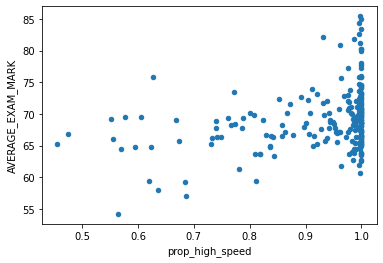
\includegraphics[scale=0.75]{prop_mark_scatter.png}
\end{figure}
    In order to address the issue in the initial model, I create a new variable PROP\_HIGH\_SPEED by combining the proportion of hexagons that have 50/10 and 25/5 access. This new variable can be interpreted as the proportion of hexagons attached to a school that have a high speed internet connection capable of supporting heavy multimedia use. Descriptive statistics shown in table ~\ref{tab:propHighSpeedSummary} indicate that while the mean connection quality is good, there is still sufficient variation to produce meaningful results. Moreover, Figure ~\ref{fig:scatterPropAverage} shows a scatter plot of PROP\_HIGH\_SPEED and AVERAGE\_HIGH\_MARK which indicates some mild correlation. The specification is therefore redefined as:
    \begin{align*}
        \text{AVERAGE\_EXAM\_MARK}_i &= \beta_0 + \beta_1(\text{PROP\_HIGH\_SPEED}_i) + \\
        & \beta_2(\text{type\_PUBLIC}_i) + \beta_3(\text{PERCENT\_ESL}_i) + \\
        & \beta_4(\text{PERCENT\_SPECIAL\_NEEDS}_i) + \\
        & \beta_5(\log(\text{MEDIAN\_INCOME}_i)) + \epsilon_i
    \end{align*}
    As before, each explanatory variable is associated to a school $i$, while $\beta_0$ is the intercept and $\epsilon_i$ is the error term. Our coefficient of interest is $\beta_1$, while the rest are controls. There is no longer significant multicollinearity, with VIF values for all coefficients under 2. Conducting a Breusch-Pagan Test still shows presence of heteroskedasticity, so robust standard errors are used.

\begin{table}[]
    \begin{threeparttable}
        \caption{OLS Regression for Aggregated Model}
        \label{tab:aggregatedModel}
        \setlength\tabcolsep{0pt} % let LaTeX figure out amount of inter-column whitespace
        \begin{tabular*}{\textwidth}{@{\extracolsep{\fill}} l *{4}{d{2.4}} }
        \toprule
            & (1) & (2) & (3) & (4)\\
        \midrule
        PROP\_HIGH\_SPEED           & 13.2113\ast\ast\ast     & 8.33536\ast\ast\ast    & 9.11846\ast\ast               & 5.988986\ast   \\
                                    & (6.640)       & (2.55533)             & (2.75994)             & (2.984493) \\
        type\_PUBLIC                &               & -7.57183\ast\ast\ast  & -7.56874\ast\ast\ast  & -5.259132\ast\ast\ast\\
                                    &               & (0.89466)             & (0.88882)             & (0.946128) \\
        LOG\_MEDIAN\_INCOME         &               &                       & -2.31635              & -2.168867 \\
                                    &               &                       & (1.37542)             & (1.379844) \\
        PERCENT\_ESL                &               &                       &                       & -0.115430\\
                                    &               &                       &                       & (0.059829)\\
        PERCENT\_SPECIAL\_NEEDS     &               &                       &                       & -0.332960\ast\ast\ast \\
                                    &               &                       &                       & (0.061431)\\
        Adjusted $R^2$              &  0.09751      & 0.4088                & 0.4131                & 0.4878\\
        \bottomrule
        \end{tabular*}
        \begin{tablenotes}
            \small
            \item N = 235 \\
            \item Robust standard errors are in parenthesis \\
            \item * $ p < 0.05$ ** $p < 0.01$ *** $p < 0.001$
        \end{tablenotes}
    \end{threeparttable}
\end{table}

    The results of this specification are presented in table ~\ref{tab:aggregatedModel}. Column (1) shows the effect of PROP\_HIGH\_SPEED only on AVERAGE\_EXAM\_MARK, and finds a statistically significant positive result at the 0.001 level. This result suggests that for any given school, if 10\% of its assigned hexagons were provided with higher bandwidth connections, AVERAGE\_EXAM\_MARK should increase by 1.3 points. While this seems small, it must be noted that AVERAGE\_EXAM\_MARK is the average across all students for each school, so an increase of 1.3 points elevates the performance of hundreds of students on average. The low $R^2$ is addressed by the addition of the type\_PUBLIC control in column (2), which boosts the variance explained to 41\% without sacrificing statistical significance on $\beta_1$. The coefficient on the public school dummy also shows a statistically significant negative result, which is once again consistent with expectations. Column (3) adds the income control which reduces the magnitude of $\beta_1$, but it is still significant. Concerningly, as before the median income coefficient is both negative and not statistically significant, implying student performance decreases with income, which is in contrast to existing literature \autocite{comfort2001}. It also does not improve the variance in the data appreciably, which is also unusual. Lastly, column (4) shows the regression with all controls added. With this final specification, the estimate on $\beta_1$ drops to 6, and is only significant at the 0.05 level. The result suggests that if 10\% of a given school's associated hexagons can be upgraded to higher speed connections, then the average exam marks are predicted to rise by 0.6 points. While this is considerably smaller, it still supports the hypothesis. Even though students may benefit overall from the additional resources accessible with higher quality connections, most of the time students are likely to be accessing textual resources on the internet, which are likely to work with nearly all bandwidth limitations. Hence when other variables are controlled, the effect of bandwidth quality is muted, but still postive and significant. 

    \section{Robustness}
    While the controls chosen are well established and behave mostly as expected, there are a few issues with the linking procedure. Since there are only 235 schools in the dataset, the analysis assumes that the all students in the surrounding region attend these schools, which is a necessary simplification due to the limited dataset. Moreover, the schools were not chosen randomly; they are the best in BC. Due to this selection bias, it is likely that these students do not represent the surrounding region as a whole, especially those attending independent schools who may be better off economically overall. This also impacts the effectiveness of the income controls, as the median income applies to the entire region of whom these students may not be representative. \\
    
    To address this issue, a dataset from Education Analytics containing exam results for every school in BC is also used, and the entire procedure is repeated \autocite{secondary2020}. This dataset was not used for the primary analysis as it lacks the \% of ESL and special needs students, which are important controls. Moreover, many schools have their results for different exams masked, so it is not possible to generate an average across all exams consistently. After restricting to valid English 12 marks only and reassigning the hexagons, the sample size is increased from 235 to 338, which is still less than the total of 575 schools in BC. The results of the aggregated model are shown in table ~\ref{tab:secondaryModel}. 
    
    While these results show similar statistically significant coefficient values for PROP\_HIGH\_SPEED, the variance explained is far lower, ranging from 0.06 - 0.12. This indicates that the explanatory power of the relationship found in the primary analysis may be particular to that sample. Moreover, while the coefficient for LOG\_MEDIAN\_INCOME is now positive, it is still not statistically signficant, which is once again unexpected. While this model is not an exact comparison to the primary specification as it restricts the scores to one exam and is missing some controls, it indicates that the effect exists, even if the exact magnitude requires more data to determine.  

\begin{table}[]
        \begin{threeparttable}
            \caption{OLS Regression for Aggregated Model using Exam Results published by BC Government}
            \label{tab:secondaryModel}
            \setlength\tabcolsep{0pt} % let LaTeX figure out amount of inter-column whitespace
            \begin{tabular*}{\textwidth}{@{\extracolsep{\fill}} l *{3}{d{2.4}} }
            \toprule
                & (1) & (2) & (3)\\
            \midrule
            PROP\_HIGH\_SPEED           & 10.6730\ast\ast\ast     & 8.61298\ast\ast\ast   & 8.50492\ast\ast\ast   \\
                                        & (1.9180)                & (1.86413)             & (2.09696)  \\
            type\_PUBLIC                &                         & -3.56784\ast\ast\ast  & -3.56799\ast\ast\ast \\
                                        &                         & (0.88768)             & (0.88851) \\
            LOG\_MEDIAN\_INCOME         &                         &                       & 0.24874  \\
                                        &                         &                       & (1.61798)  \\
            Adjusted $R^2$              &  0.05744                & 0.1211                & 0.1185 \\
            \bottomrule
            \end{tabular*}
            \begin{tablenotes}
                \small
                \item N = 338 \\
                \item Robust standard errors are in parenthesis \\
                \item * $ p < 0.05$ ** $p < 0.01$ *** $p < 0.001$
            \end{tablenotes}
        \end{threeparttable}
\end{table}
    
    \section{Conclusion}
    The results suggest that increasing broadband quality has a positive and significant effect on student academic performance, although it is limited in scope due to the availability of data and counter-intuitive effects discovered on some coefficients. Crucially, this study demonstrates the feasibility of linking bandwidth data to academic performance, and indicates that the quality of connection additionally impacts educational outcomes even if access is established. \\
    As a regression model is used to establish this relationship, it is not possible to conclusively show causality. While the controls are chosen from existing literature and generally behave as expected, they only confirm the existence of a statistically significant correlation. Moreover, this correlation can only be associated with performance on language arts exams, and may not generalise to other subjects. Future studies with access to time series data may be able to analyse on how student performance changes as bandwidth increases, which would better show causality. Addtionally, access to cleaner data that can directly connect a student to their exam performance and connection quality along with other controls would greatly reduce the error caused by roughly linking schools to bandwidth markers. \\
    Policy decisions regarding broadband infrastructure investment should consider this effect, as expansions and upgrades are conducted with financial assistance from the government. Directing investment away from upgrading exisiting high quality connections and towards ensuring that all students have generally good quality connections may be fruitful. Investment in high speed satellite networks would also achieve this aim, and could lead to improved student performance. 

    \clearpage
    \printbibliography
\end{document}